\documentclass[dvisvgm,tikz,border=4pt]{standalone}
\usepackage{amsmath,amssymb}
\usepackage{pgfplots}\pgfplotsset{compat=1.18}\usepgfplotslibrary{polar}
\usetikzlibrary{arrows.meta,positioning,automata,shapes,shapes.misc,calc,decorations.pathmorphing,decorations.markings,angles,quotes,patterns,mindmap,matrix,knots,hobby,trees}
\tikzset{->-/.style={decoration={markings, mark=at position 0.5 with {\arrow{Stealth}}}, postaction={decorate}}}
\begin{document}
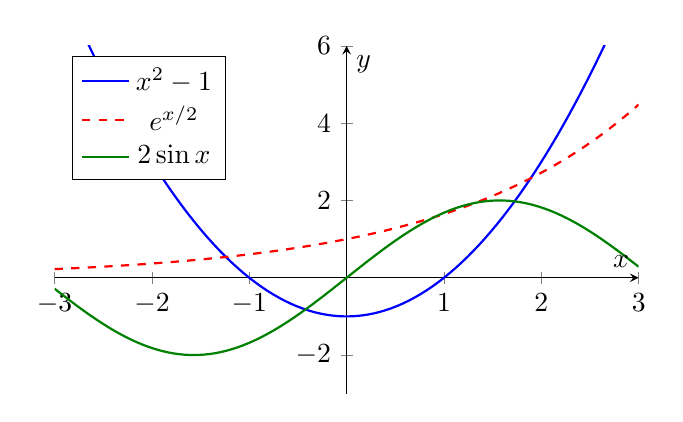
\begin{tikzpicture}
\begin{axis}[axis lines=middle, xlabel=$x$, ylabel=$y$, domain=-3:3, samples=100, legend pos=north west, width=9cm, height=6cm, ymin=-3, ymax=6]
\addplot[blue, thick] {x^2 - 1}; \addlegendentry{$x^2-1$}
\addplot[red, dashed, thick] {exp(x/2)}; \addlegendentry{$e^{x/2}$}
\addplot[green!50!black, thick] {2*sin(deg(x))}; \addlegendentry{$2\sin x$}
\end{axis}
\end{tikzpicture}
\end{document}
